\documentclass[12pt]{article}
\usepackage[english]{babel}
\usepackage{natbib}
\usepackage{url}
\usepackage[utf8x]{inputenc}
\usepackage{amsmath}
\usepackage{graphicx}
\graphicspath{{images/}}
\usepackage{parskip}
\usepackage{fancyhdr}
\usepackage{vmargin}
\usepackage{xcolor}
\usepackage{siunitx}
\usepackage{physics}
\usepackage{subcaption}




\setmarginsrb{3 cm}{2 cm}{3 cm}{2 cm}{1 cm}{1.5 cm}{1 cm}{1.5 cm}

\title{Lab 03}													% Title
\author{G 03}														% Author
\date{2 Apr 2019}														% Date

\makeatletter
\let\thetitle\@title
\let\theauthor\@author
\let\thedate\@date
\makeatother

\pagestyle{fancy}
\fancyhf{}
\rhead{\theauthor}
\lhead{\thetitle}
\cfoot{\thepage}
\newcommand{\mis}[3]{(#1 \pm #2) \ #3}
\newcommand{\misp}[3]{(#1 \#3 \pm #2}
\begin{document}

%%%%%%%%%%%%%%%%%%%%%%%%%%%%%%%%%%%%%%%%%%%%%%%%%%%%%%%%%%%%%%%%%%%%%%%%%%%%%%%%%%%%%%%%%

\begin{titlepage}
	\centering
    \vspace*{0.5 cm}
    
\includegraphics[scale = 0.75]{polito.jpg}\\[1.0 cm]				% University Logo
    \textsc{\LARGE Politecnico di Torino}\\[2.0 cm]						% University Name
	\textsc{\Large Digital systems electronics\\ A.A. 2018/2019}\\[0.5 cm]		% Course Code
	\textsc{\Large Prof. G. Masera}\\[0.5 cm]		% Nome del Professore
	\rule{\linewidth}{0.2 mm} \\[0.4 cm]
	{ \huge \bfseries \thetitle \\ \small \thedate}\\
	\rule{\linewidth}{0.2 mm} \\[1.5 cm]
	
	\begin{minipage}{0.4\textwidth}
		\begin{flushleft} \large
			Berchialla Luca\\												%Cognomi e nomi
			Laurasi Gjergji
			\\
			
			Mattei Andrea\\
            Lombardo Domenico Maria\\
            
			\end{flushleft}
			\end{minipage}~
			\begin{minipage}{0.4\textwidth}
            
			\begin{flushright} \large
			236032\\													%Matricole
			238259\\
            233755\\
            233959\\
            
		\end{flushright}
        
	\end{minipage}\\[2 cm]
	
\end{titlepage}

%%%%%%%%%%%%%%%%%%%%%%%%%%%%%%%%%%%%%%%%%%%%%%%%%%%%%%%%%%%%%%%%%%%%%%%%%%%%%%%%%%%%%%%%%

\section{4-bit Sequential RCA}
\subsection{Implementation}

\begin{figure}[h]
	\centering
	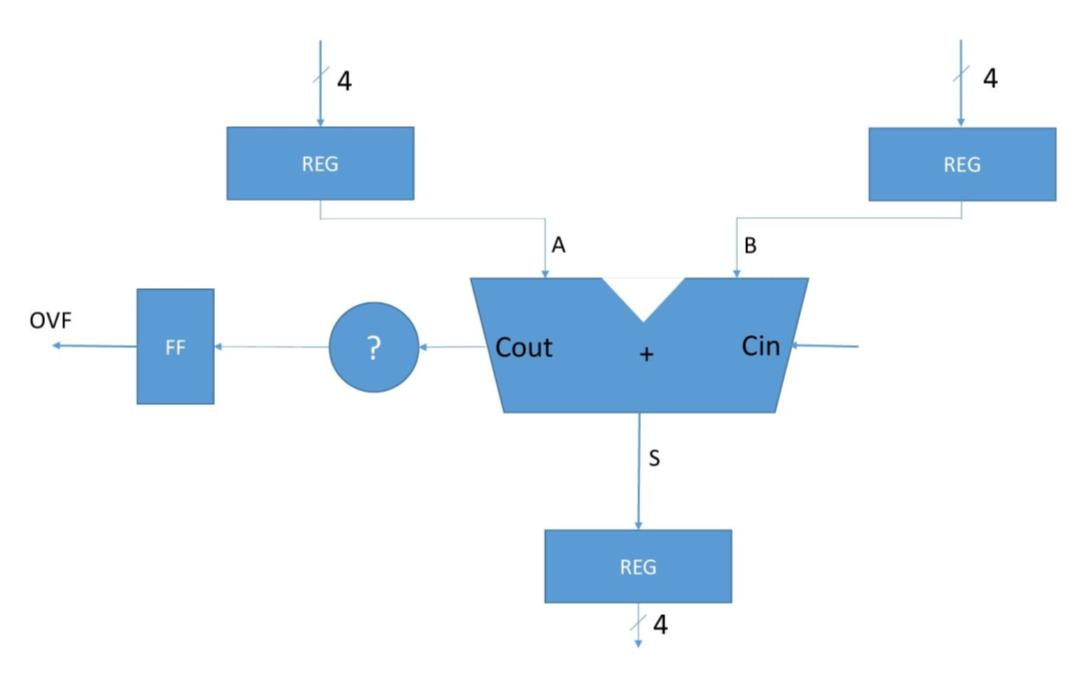
\includegraphics[scale = 0.8]{immagini/B1.jpg}
	\caption{Top level entity}
\end{figure}


Here we had to implement a 4-bit Sequential Ripple Carry Adder. To build the circuit requested in $figure 1$ several sub-circuits have been implemented.\\
As first point a Full Adder was implemented as shown in $figure$ $2a$. The 4-bit adder was built using four full adders in a ripple carry architecture. Its overflow signal is generated by a $xor$ gate whose inputs are the $carry_{out}$ signals of the last two full adders.\\

\begin{figure}[h]
	\centering
	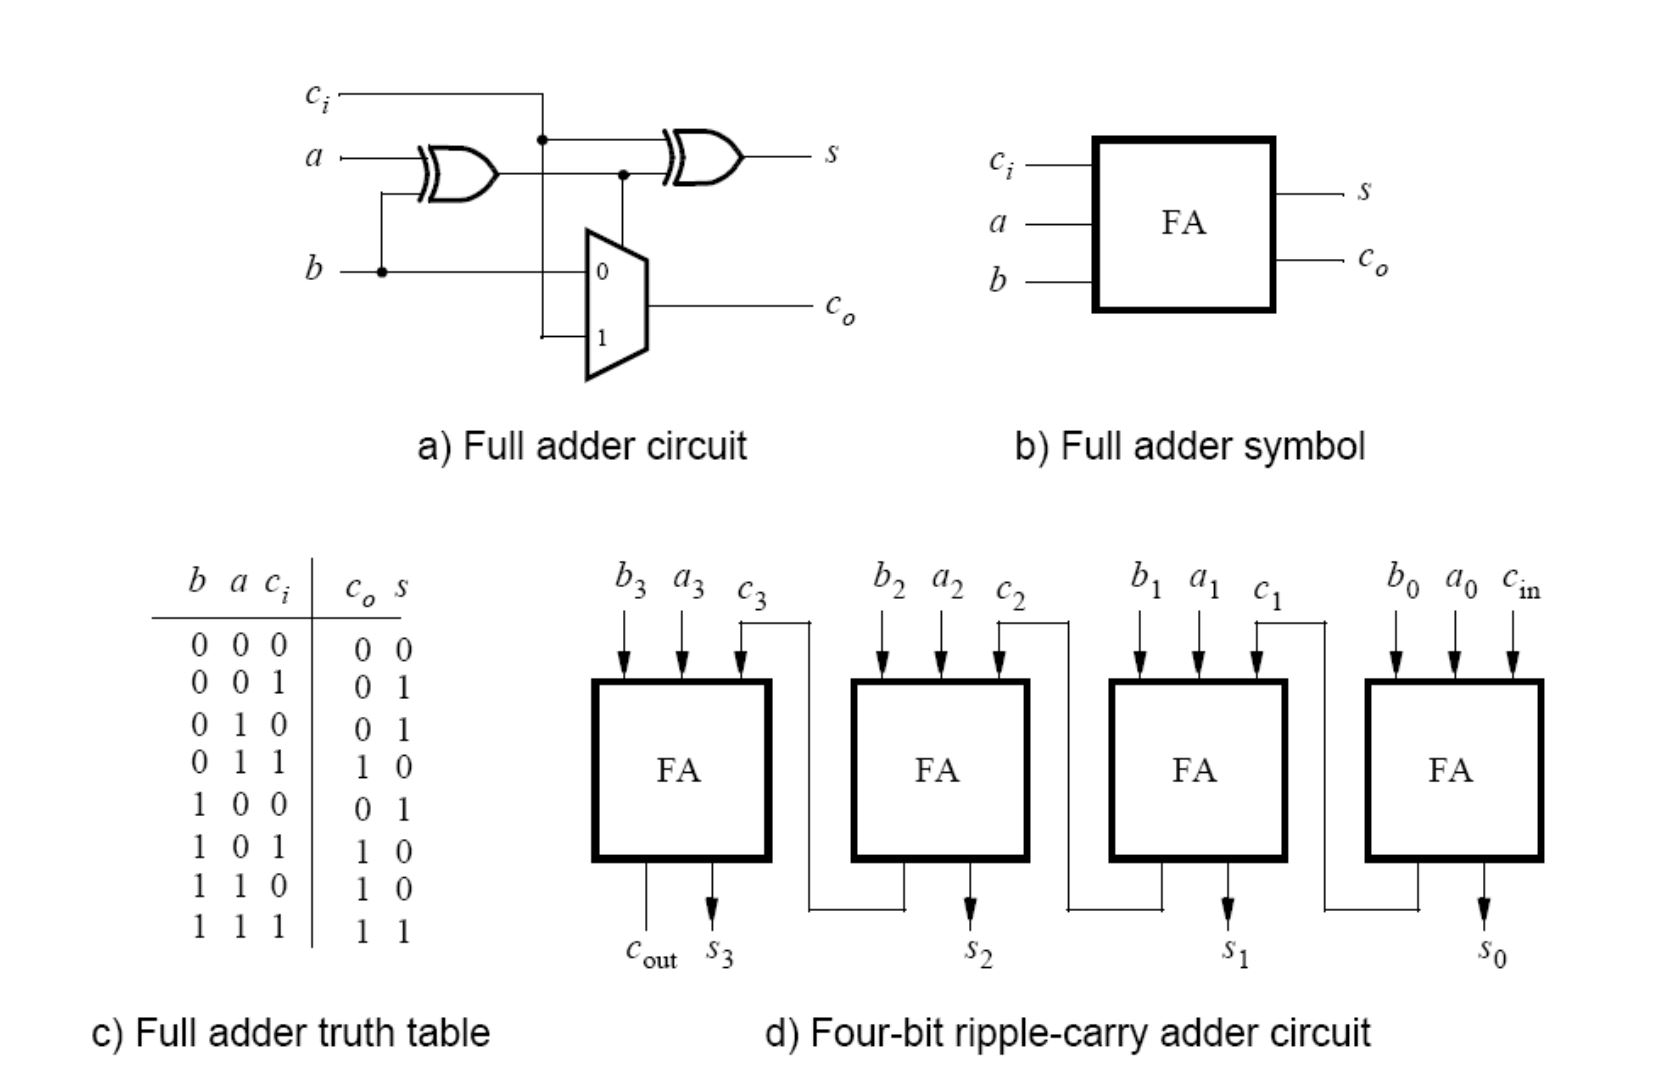
\includegraphics[scale = 0.4]{immagini/B2.jpg}
	\caption{Full Adder}
\end{figure}

The Register and the Flip-Flop were implemented using the code provided in the instructions.\\
A new 7-segments display decoder was needed in order to display properly 2's complement numbers. It uses two 7-segments displays to show respectively the sign and the magnitude of the number. The implementation was done by means of the $when-else$ statement following the truth table in $figure$ $3$.
\begin{figure}[h]
	\centering
	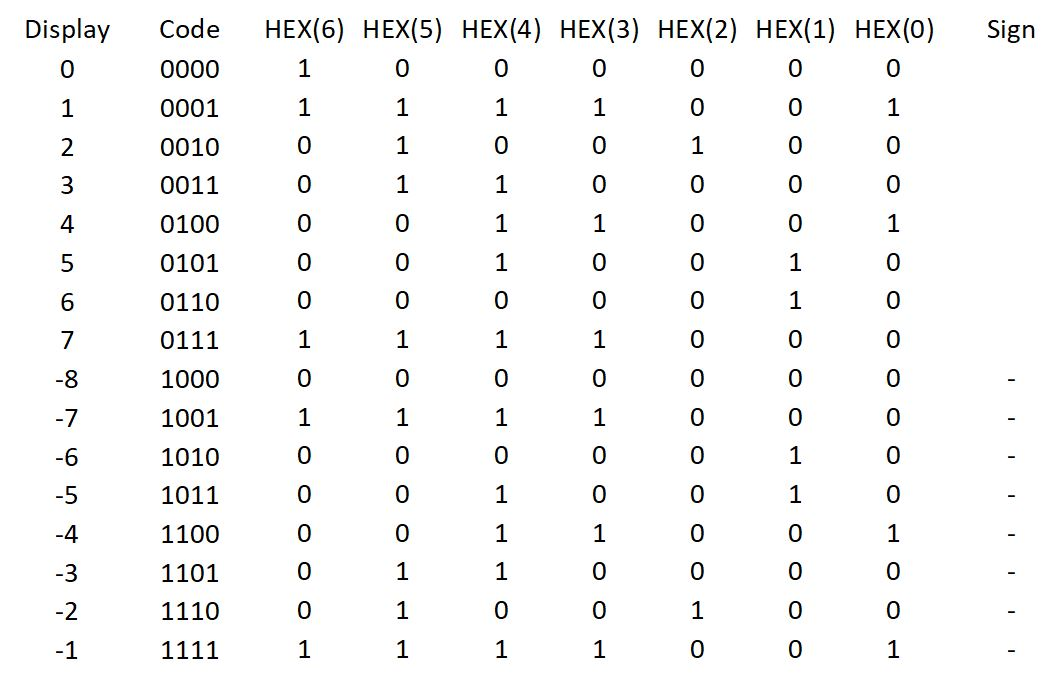
\includegraphics[scale = 0.7]{immagini/B3.jpg}
	\caption{2's complement 7-segments decoder}
\end{figure}\\
The top level entity that implements the circuit is in the file $lab3\_es1.vhd$ where all the components needed are instantiated and connected together.\\ As required, the the inputs $A$ and $B$ have been assigned to $SW_{3-0}$ and $SW_{7-4}$ respectively, $KEY_0$ to the negated asynchronous reset input and $KEY_1$ to the clock. The magnitude and the sign of $A$ are displayed in $HEX4$ and $HEX5$ respectively. The same is done for $B$ and $S$ in $HEX2,HEX3$ and $HEX0,HEX1$ respectively. The adder's overflow is shown by means of the red $LEDR_9$.\\

\subsection{Testbench}
To validate the correct behavior of the circuit a testbench was created. The $clock$ signal was created using a process and its period has been fixed to $10ps$, the reset signal instead has a period of $115ps$, not a multiple of the clock, to verify that is asynchronous. It  is active for $10ps$ and is generated just 10 times in order to have cleaner waveforms.\\
To test every possible combination of inputs it has been used a 8-bit counter which increments its value every $100ps$, the least significant 4 bits have been assigned to $A$ and the others to $B$.\\
Since the the values of $A,B$ and $S$ coded for the 7-segments display are the output of the circuit in the testbench are present several if clauses that  translate the output values to the 2's complement binary value of $A,B$ and $S$.\\
\\
\subsection{Timing analysis}
The maximum operating frequency of the circuit $f_{max}$ has been determined with the help of Quartus Prime and TimeQuest and is $f_{max}=650MHz$.\\
The longest path in the circuit in terms of delay is the one that starts from the MSB of a register where $A$ or $B$ are stored and arrives to the Flip Flop that stores the overflow signal. This path is longer than the other possible path that starts from one of the previous registers and arrives to the register where $S$ is stored, because the overflow signal is calculated by a $xor$ gate whose inputs are the $carry_{out}$ signals of the last two full adders. Therefore, with respect to the MSB of $S$, which goes directly to the register, the signal has to be processed by the $xor$ gate before arriving to the flip flop.


\section{4-bit Sequential Adder/Subtractor}
\subsection{Implementation}
The circuit implemented in this section is a little modification of the circuit implemented in section 1. In particular the  4-bit full adder has been modified to make it perform also the subtraction. The $carry_{in}$ input is replaced by the $add_subtract$ input  that enables the sum when its value is $0$ and the subtraction when is $1$. The $B$ input is 2's complemented when $add_subtract=1$ by assigning the $B_i$ input of each full adder to the xor of $B_i$ and $add_subtract$ and by assigning the $carry_{in}$ of the first full adder to $add_subtract$.\\ 
\subsection{Testbench}
The $add_subtract$ input was then assigned to $SW_8$ in the top level entity. In the testbench the counter has been modified now being 9-bit wide and its MSB is assigned to $add_subtract$.\\ 
\subsection{Timing analysis}
The maximum operating frequency of the circuit $f_{max}$ has been determined  as in section 1 and its value is $f_{max}=600MHz$. $f_{max}$ is lower for this circuit because the longest path now includes another level of logic that  is between the output of the register where $B$ is stored and the input of the full adder. \\
Therefore the longest path is the same as the previous section but it starts only from the previously mentioned register because only between  it and the full adder there are the additional $xor$ gates.\\

%%%%%%%%%%%%%%%%%%%%%%%%%%%%%%%%%%%%%%%%%%%%%%%%%%%%%%%%%%%%%%%%%%%%%%%%%%%%%%%
\newpage
\section{ 16-bit RCA, Carry-Bypass Adder and Carry-Select Adder }

In this section will be presented three different implementations of 16 bit adders. 
Each of them will be simulated by means of a testbench, timing analysis will be performed as well. 
The different adders are tested over the same circuit architecture shown in the next $figure$. The 16-bit adder receives the 2 16-bit addends from 2 registers and sends the summing result to a third register. Finally the result and the addends are decoded into hexadecimal values.
\newline
\newline

\begin{figure}[h]
	\centering
	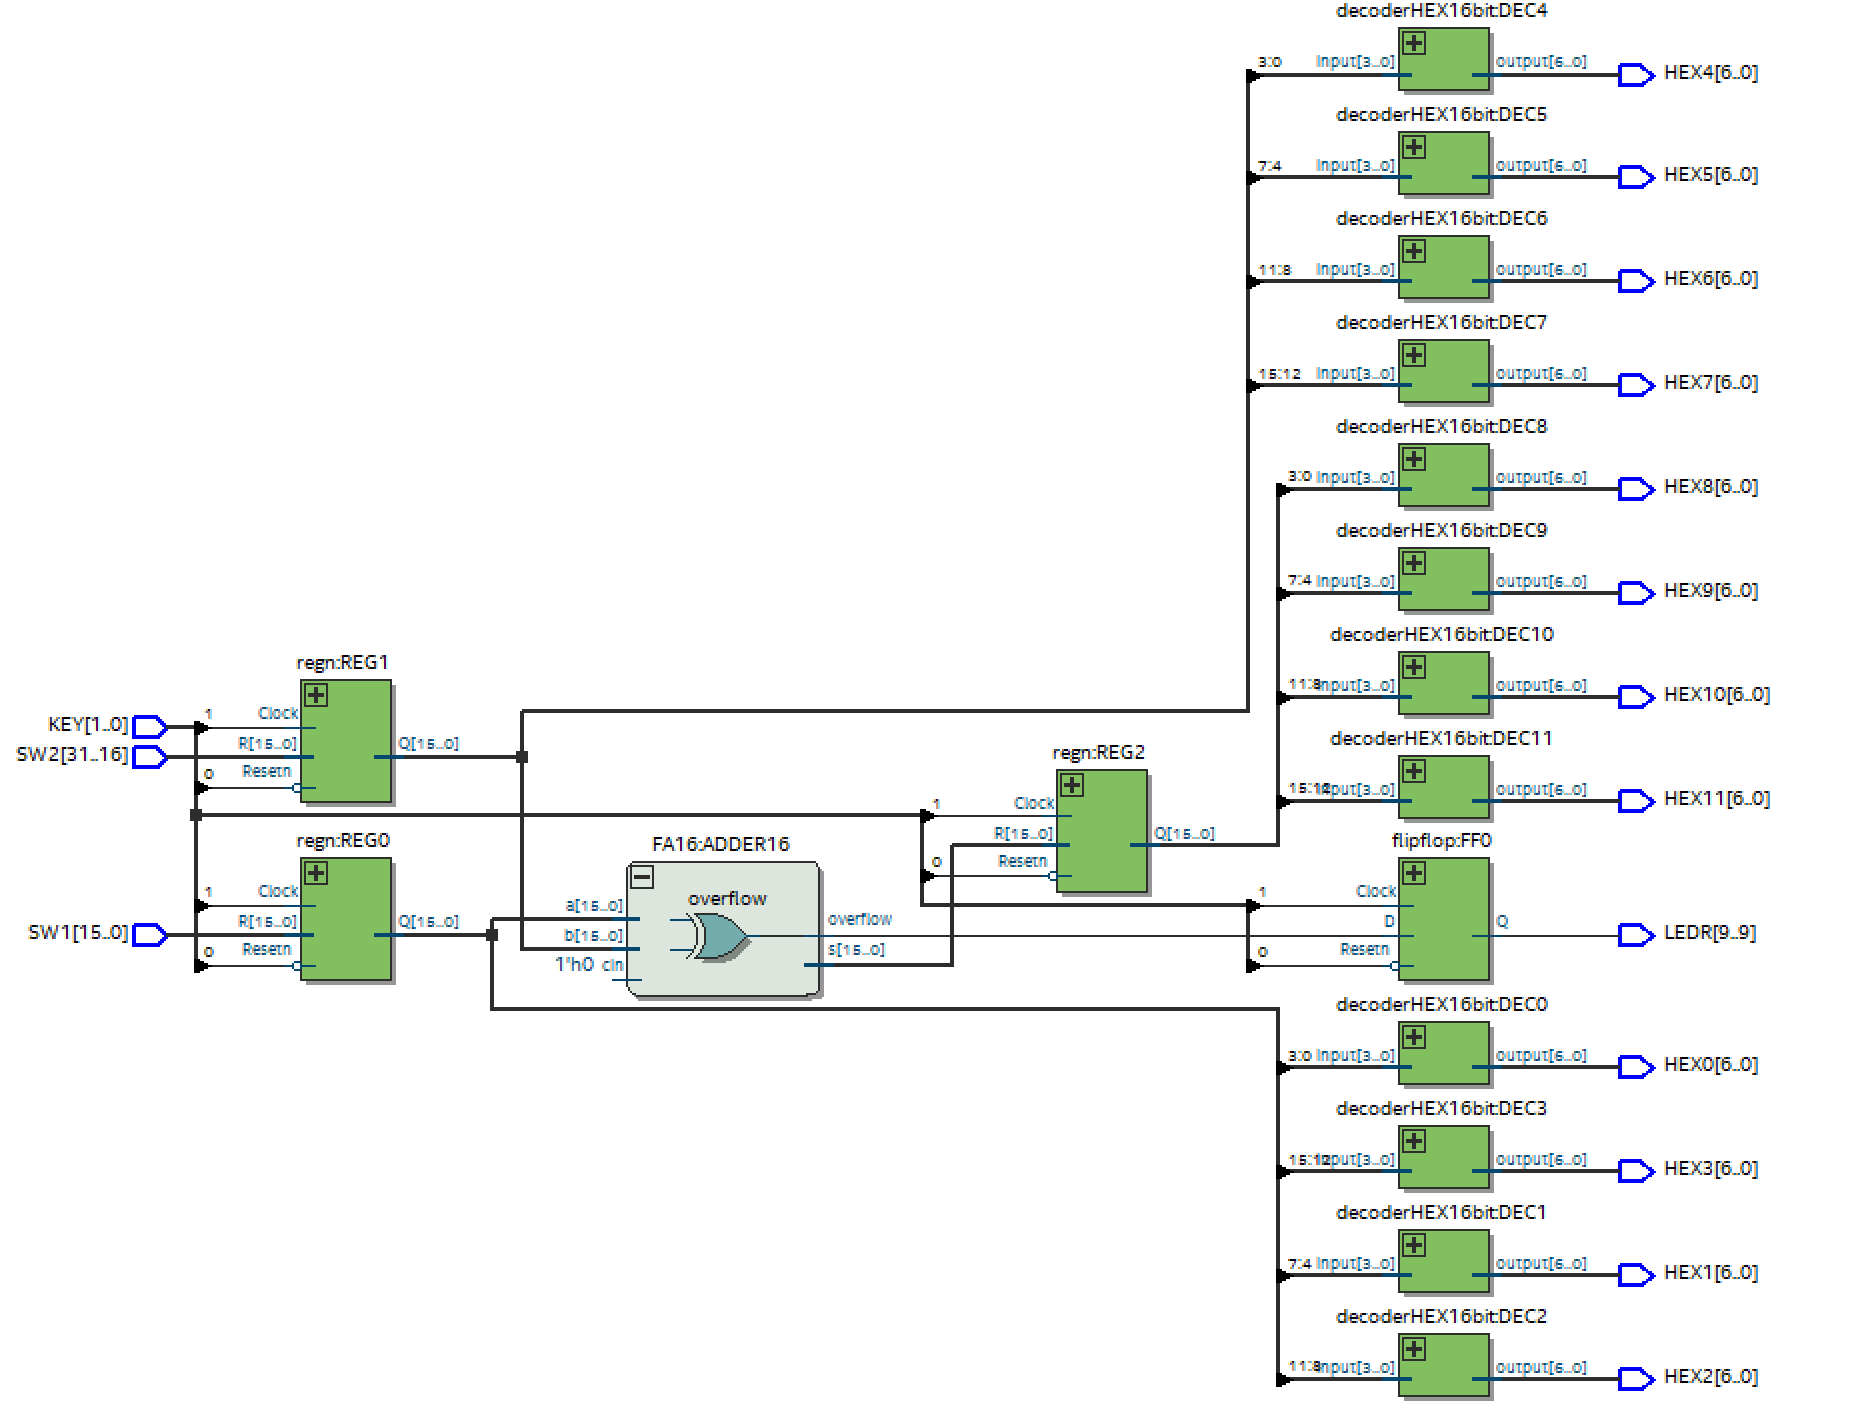
\includegraphics[scale = 0.6]{immagini/niki/rtlgeneral.png}
	\caption{Architecture of the circuit including the general 16-bit adder}       
	
\end{figure}
\newpage
\subsection{16-bit RCA}

The first implemented architecture is the classical Ripple Carry Adder (RCA).
As shown in the figure below the carry output of each FA becomes the carry input of the next FA. 
 \begin{figure}[!h]
 	\centering
 	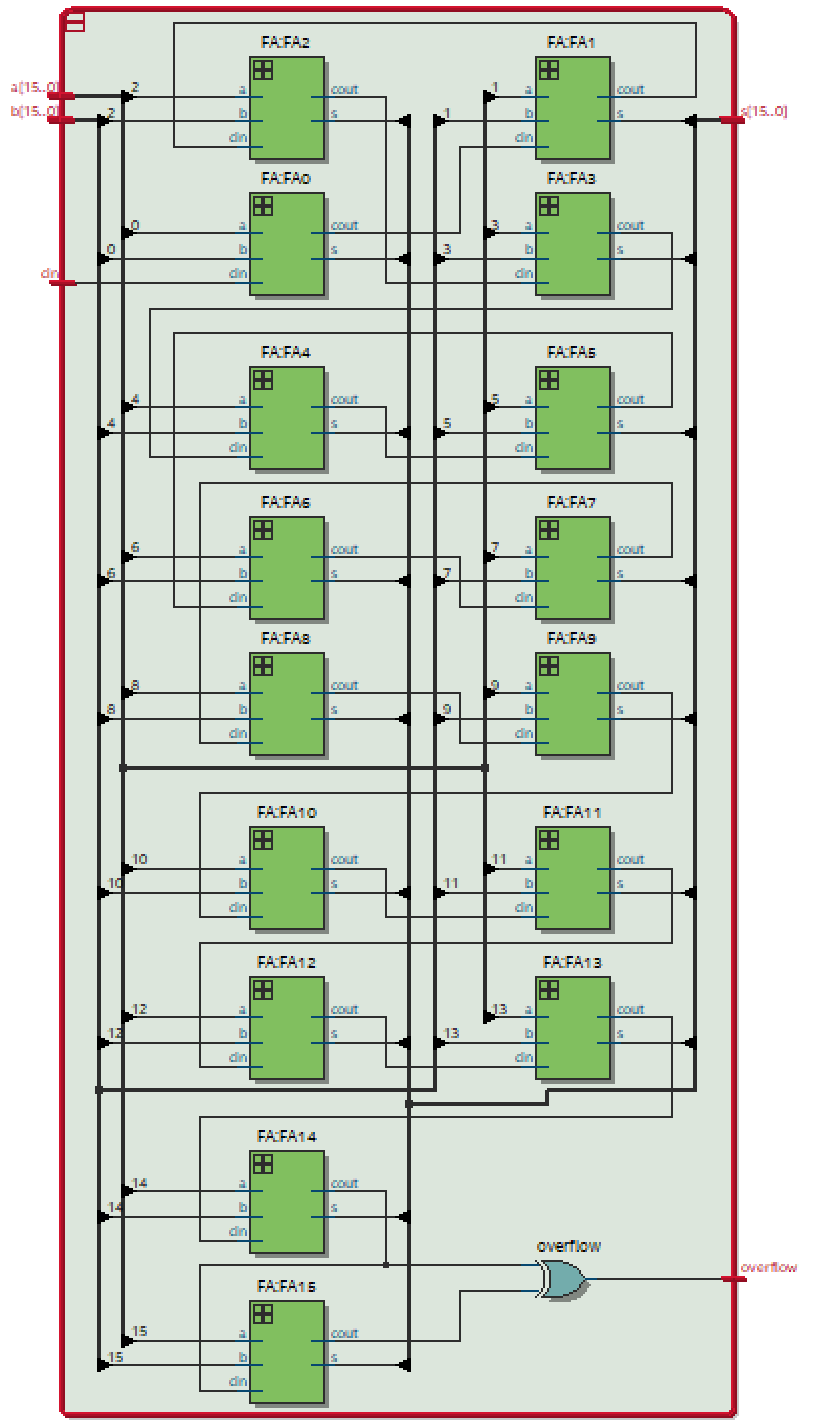
\includegraphics[scale = 0.6]{immagini/niki/rtl2_a.png}
 	\caption{RCA adder architecture}       
 \end{figure}

The resulting thestbench is shown in the next image.

 \begin{figure}[!h]
	\centering
	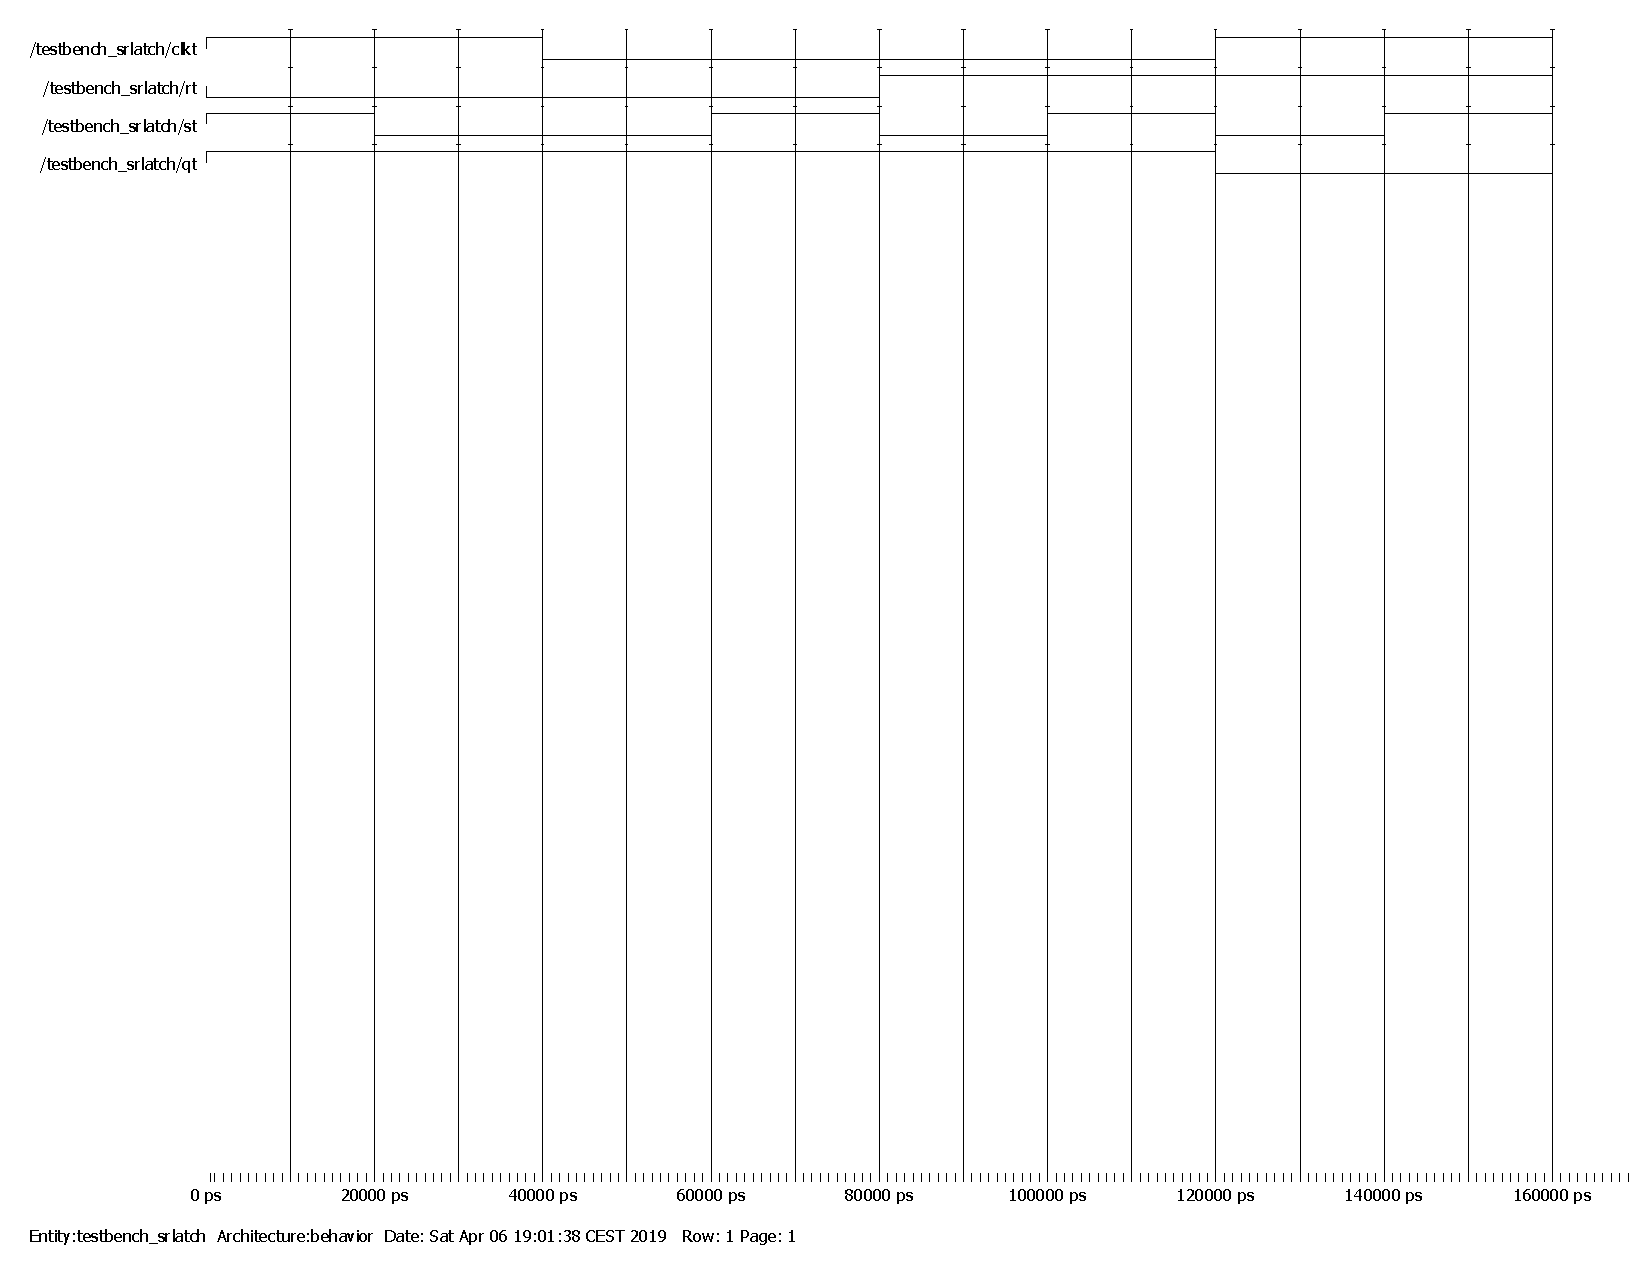
\includegraphics[scale = 0.55]{immagini/niki/testbench1.png}
	\caption{RCA testbench}       
\end{figure}
\newpage
The quartus timing analysis tool gives the results:
 \begin{figure}[!h]
 	\centering
 \begin{subfigure}{\linewidth}	
 	\centering
 		\raisebox{1cm}{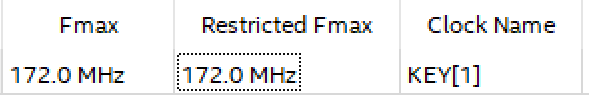
\includegraphics[scale = 0.8]{immagini/niki/f2.png}}
 	\raisebox{0.4mm}{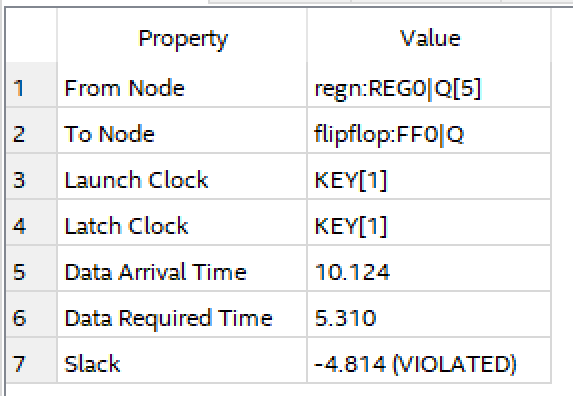
\includegraphics[scale = 0.7]{immagini/niki/delay2.png}} 	
 \end{subfigure}

\end{figure}

meaning that the worst-case delay path is $5.814 ns $ long, corresponding to a maximum usable frequency of $172MHz$.

\subsection{16-bit Carry Bypass adder}

The circuit shown below implements a 16-bit carry bypass adder. This architecture creates an alternative path for the carry of each block of full adders. If the output carry equals the input carry then it might be propagated resulting in a faster operation.
\begin{figure}[!h]
	\centering
	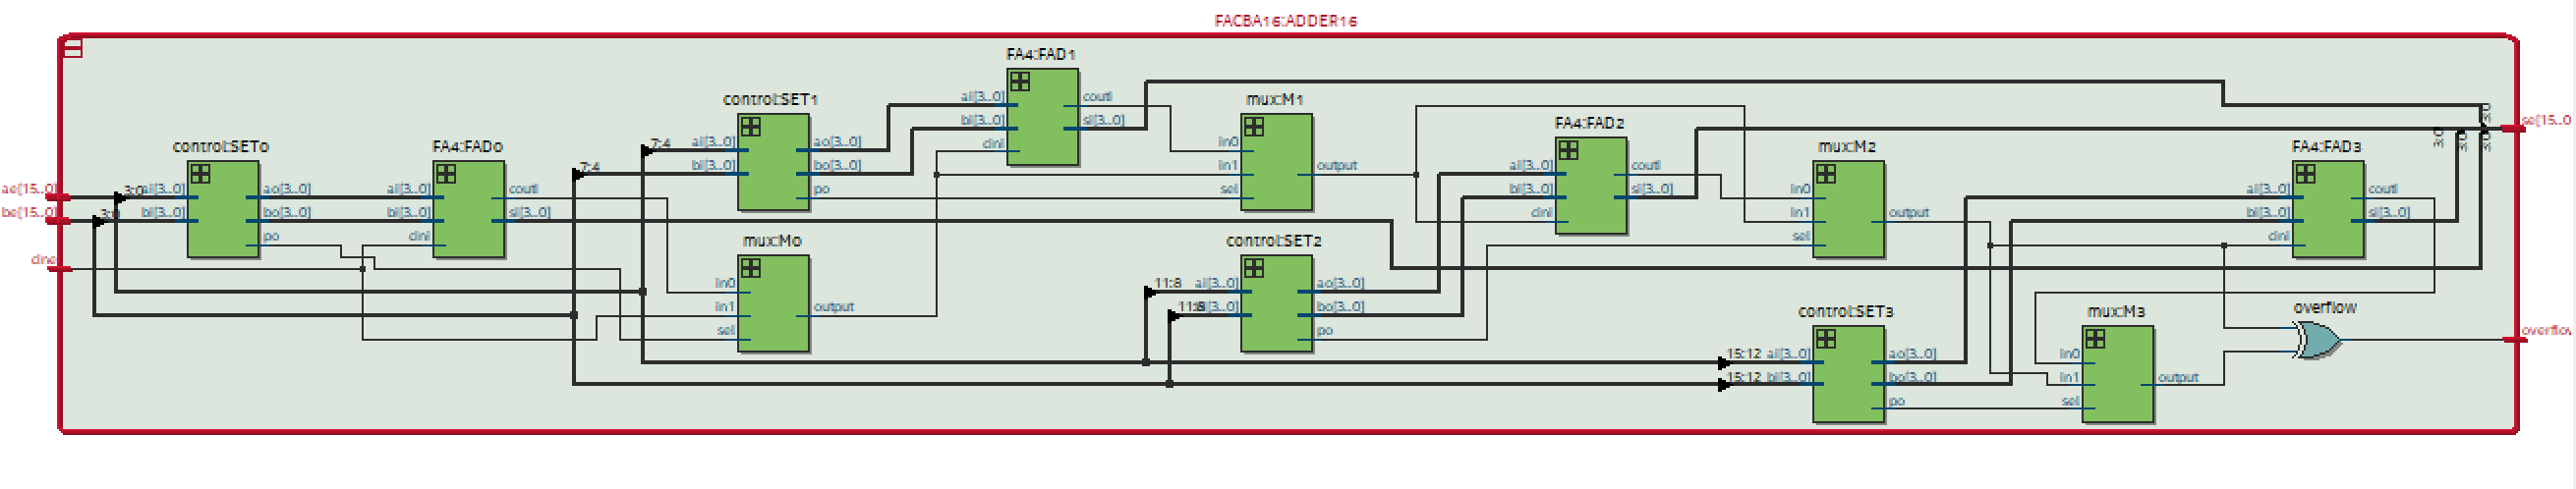
\includegraphics[scale = 0.45]{immagini/niki/parte2_rtl.png}
	\caption{16-bit Carry Bypass Adder}       
\end{figure}

The control blackbox shown below checks the condition of carry propagation enabling a MUX that select the right carry path.

\begin{figure}[!h]
	\centering
	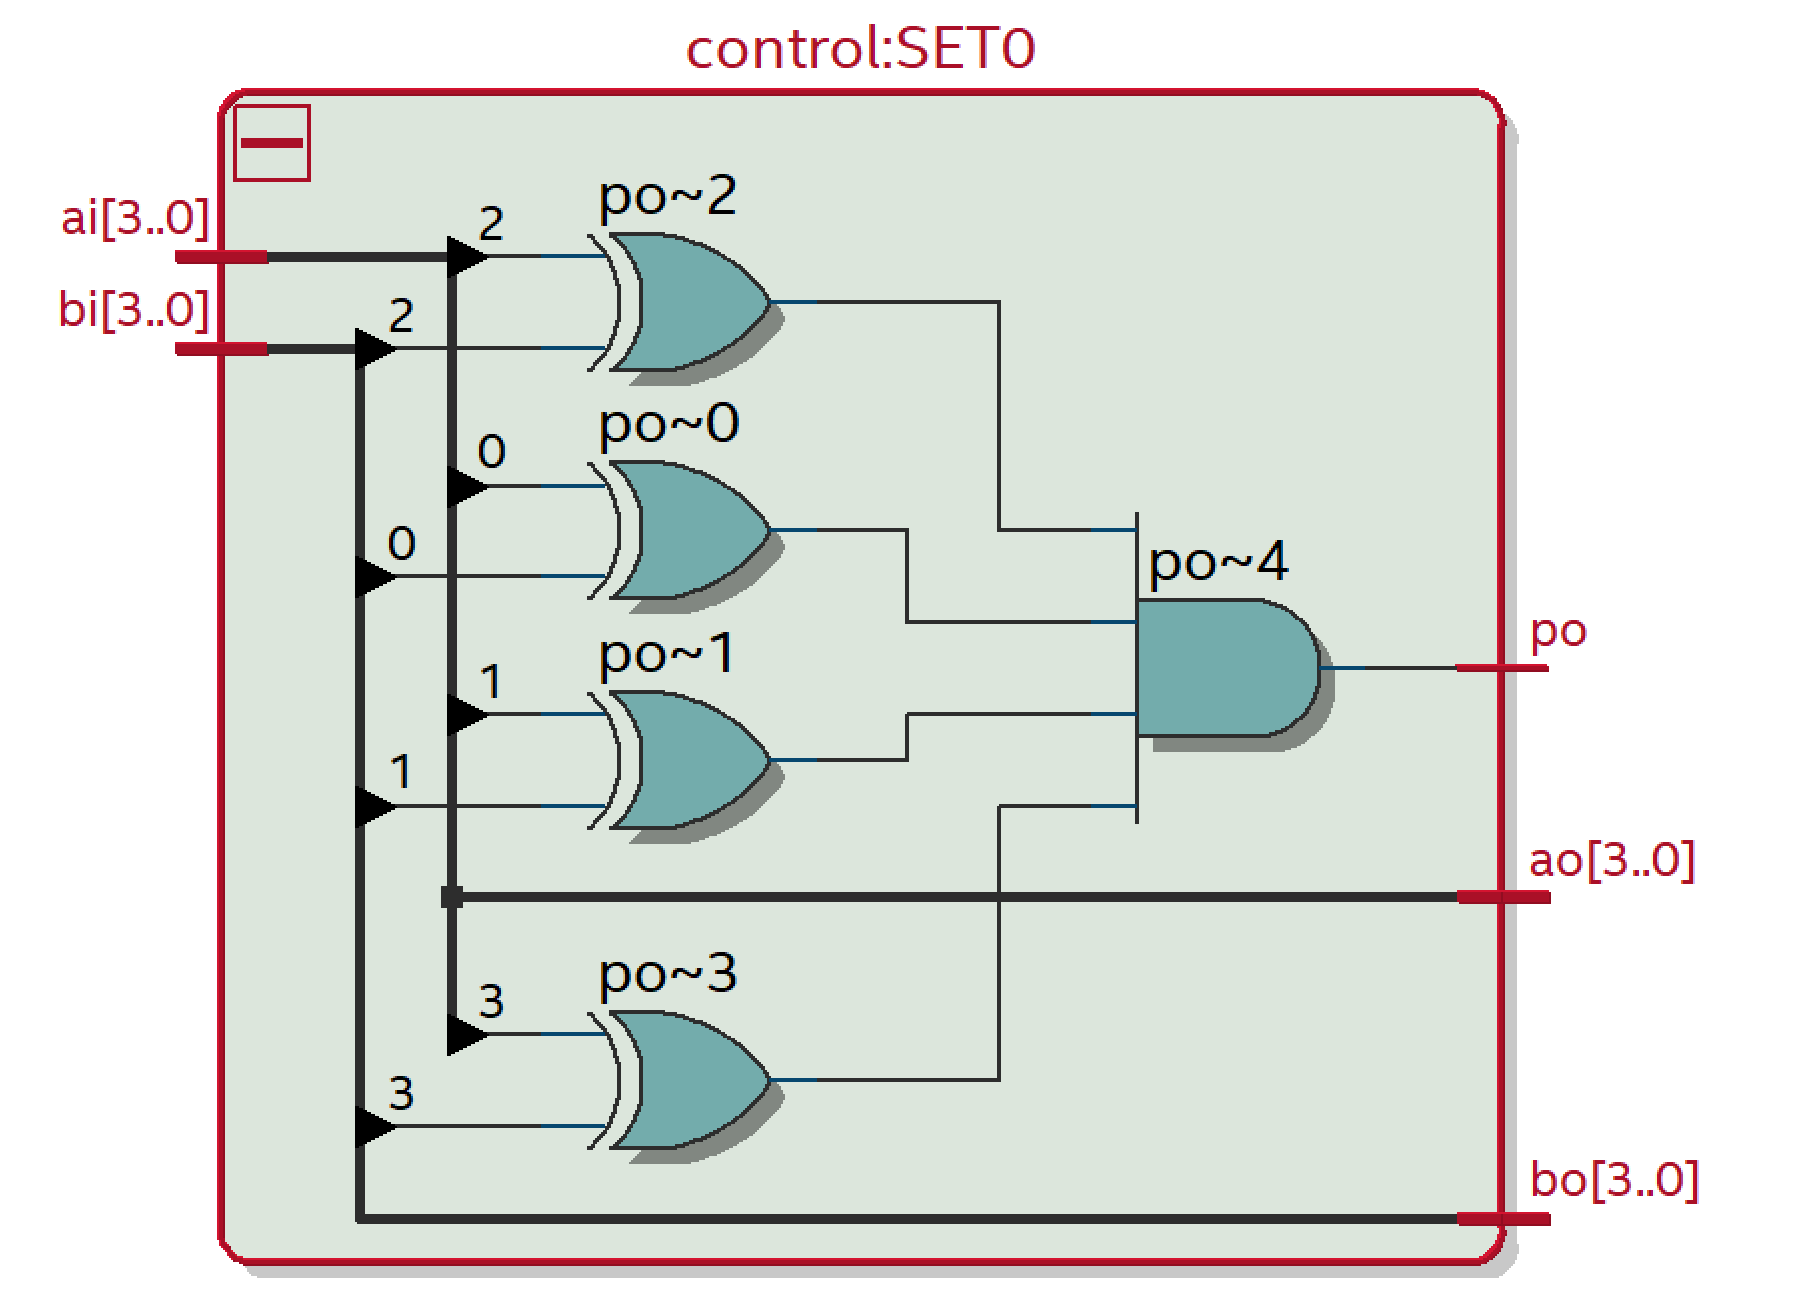
\includegraphics[scale = 0.2]{immagini/niki/rtl2.png}
	\caption{control blackbox}       
\end{figure}
\newpage
As before a testbench has been generated validating the design:

\begin{figure}[!h]
	\centering
	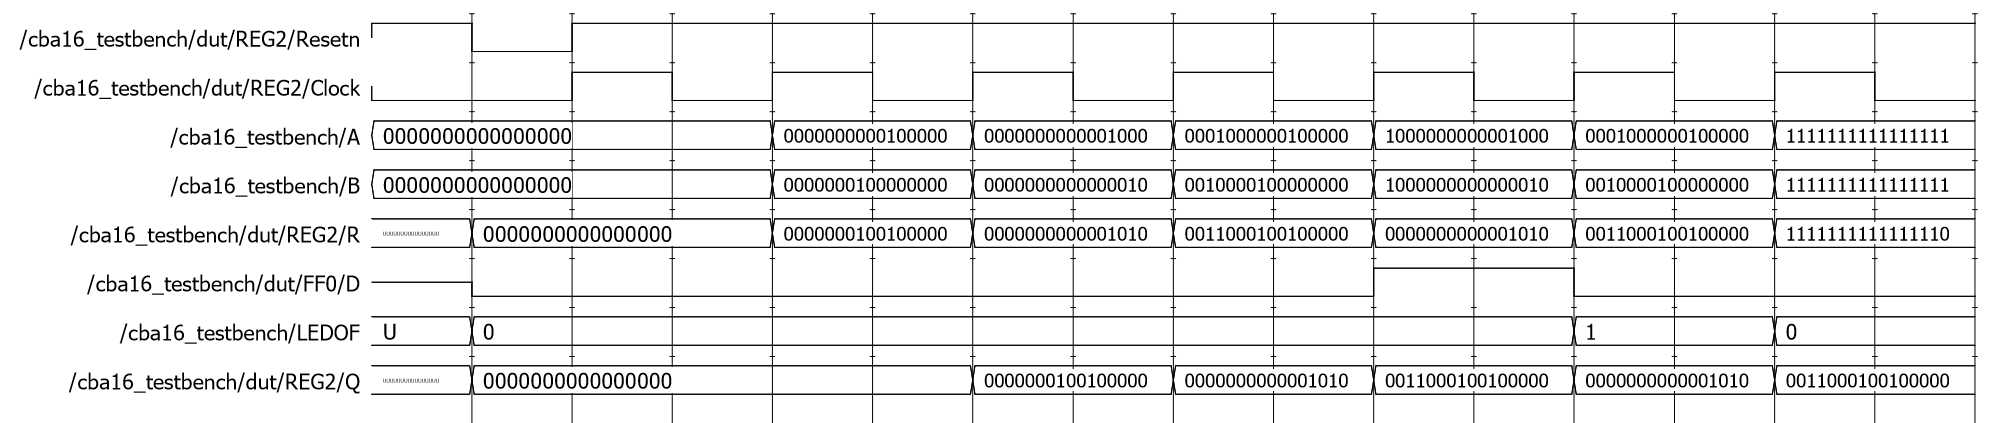
\includegraphics[scale = 0.58]{immagini/niki/testbench2.png}
	\caption{CBA testebench}       
\end{figure}

This time quartus timing analysis tool returns the results:
\begin{figure}[!h]
	\centering
	\begin{subfigure}{\linewidth}	
		\centering
		\raisebox{1cm}{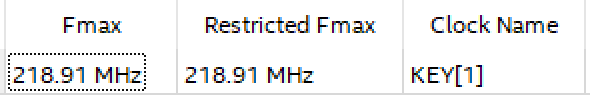
\includegraphics[scale = 0.9]{immagini/niki/f3.png}}
		\raisebox{0.4mm}{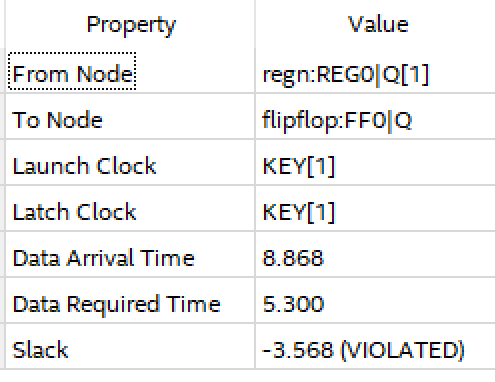
\includegraphics[scale = 0.8]{immagini/niki/delay3.png}} 	
	\end{subfigure}
	
\end{figure}

meaning that the worst-case delay path is $4.568 ns $ long, corresponding to a maximum usable frequency of $218.91MHz$, much higher than the first architecture.

%%%%%%%%%%%%%%%%%%%%%%%%
\newpage
\subsection{16-bit Carry Select Adder}

The circuit shown below implements a 16-bit carry select adder. This time the architecture doubles the number of FAs calculating the possibile results for each possible carry input condition. 
At the end the true result is generated using a set of MUX that select the 'already calculated' result corresponding to the given carry input. 
\begin{figure}[!h]
	\centering
	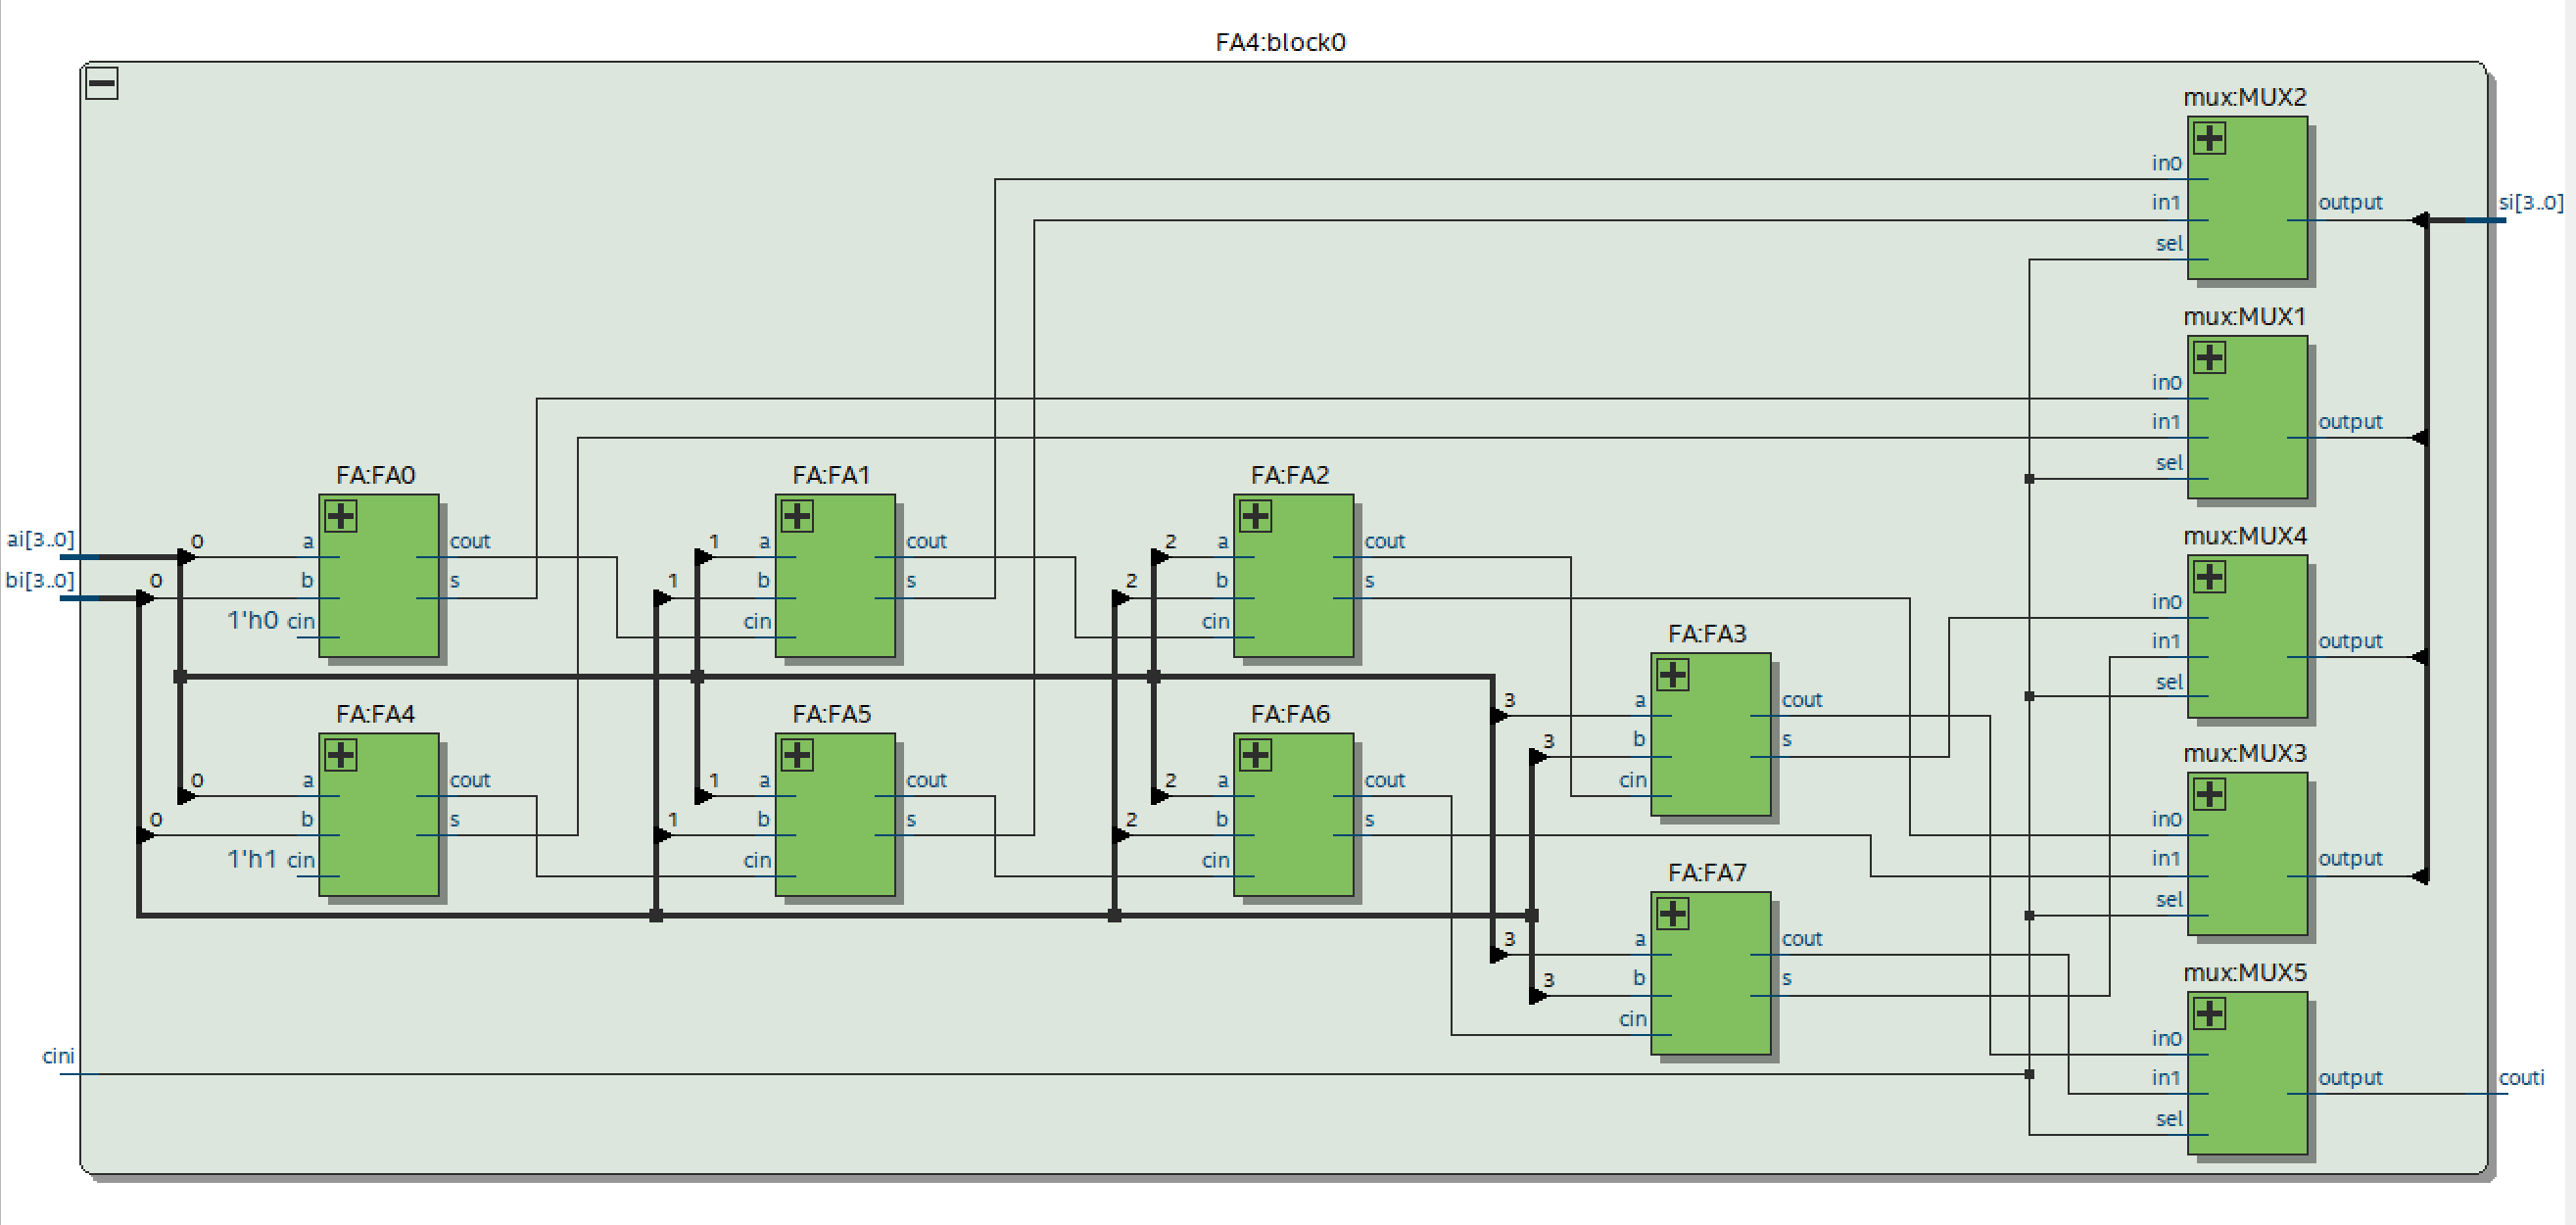
\includegraphics[scale = 0.4]{immagini/niki/rtl3.png}
	\caption{16-bit Carry Select adder }       
\end{figure}

As before a testbench has been generated validating the design:

\begin{figure}[!h]
	\centering
	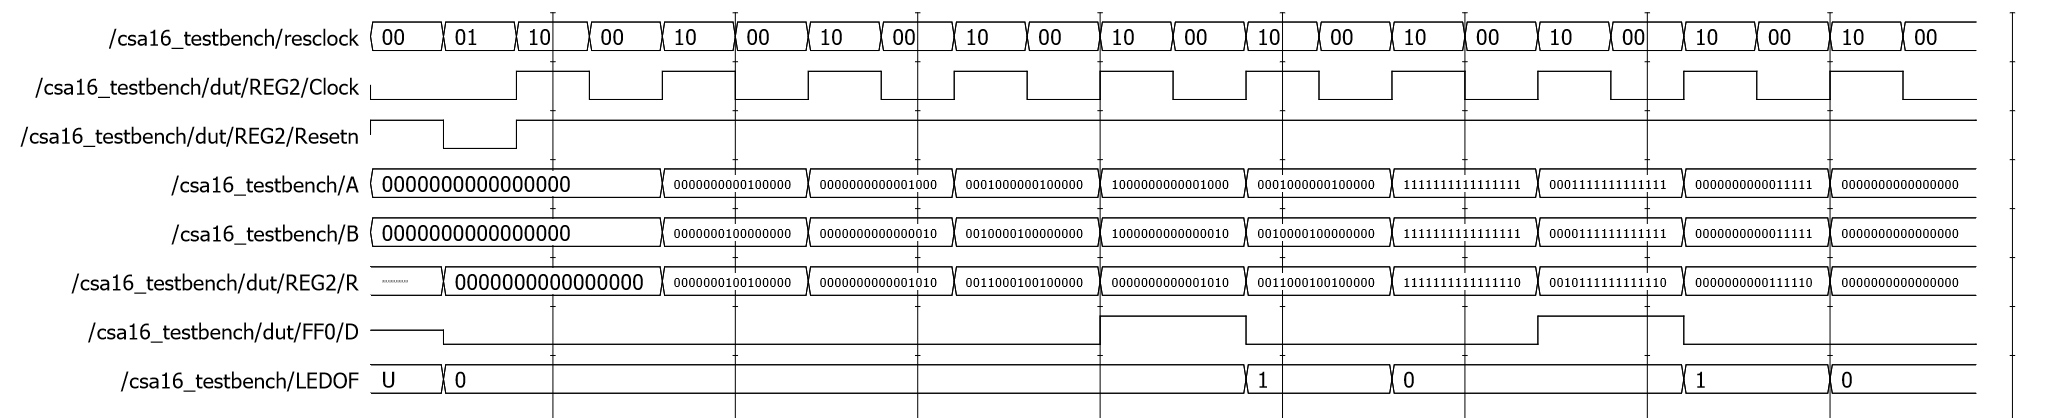
\includegraphics[scale = 0.58]{immagini/niki/testbench3.png}
	\caption{16-bit CSA testebench}       
\end{figure}
\newpage

This time quartus timing analysis tool returns the results:
\begin{figure}[!h]
	\centering
	\begin{subfigure}{\linewidth}	
		\centering
		\raisebox{1cm}{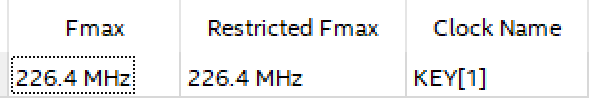
\includegraphics[scale = 0.9]{immagini/niki/f1.png}}
		\raisebox{0.4mm}{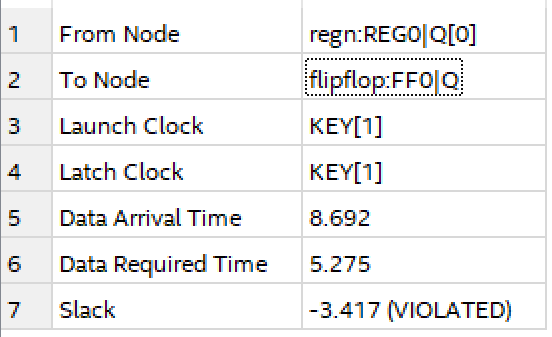
\includegraphics[scale = 0.8]{immagini/niki/delay1.png}} 	
	\end{subfigure}
	
\end{figure}

meaning that the worst-case delay path is $4.417 ns $ long, corresponding to a maximum usable frequency of $226.4MHz$,
this result is similar to the CBA adder but still the implemented 16-bit CSA returns the fastest results.
 



%%%%%%%%%%%%%%%%%%%%%%%%%%%%%%%%%%%%%%%%%%%%%%%%%%%%%%%%%%%%%%%%%%%%%%%%%%%%%%%
\newpage
\section{Multiplier}

The task of this part of the experience is design a 4-bit multiplier using VHDL, the circuit implemented is based on the one in $Figure$ $4$. 
\begin{figure}[h]
	\centering
	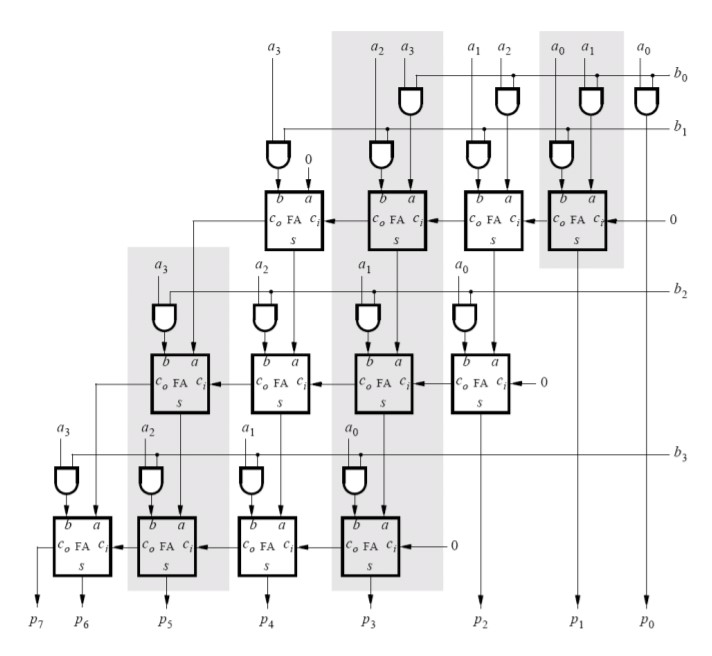
\includegraphics[scale = 0.4]{immagini/multiplier-circuit.jpg}
	\caption{the circuit implemented for the multiplier}       

\end{figure}
The input of the circuit are the DE10 switch from 0 to 7, the first four represent the first number while the remaining compose the second number.
The output of the circuit are the first 4 seven-segments displays of the board that are used for displaying hexadecimal numbers. The first 2 displays show the 2 operands while the other 2 display the result.
The overall architecture ($Figure$ $5$) of the circuit is composed by the multiplier (multiplier.vhd) and 4 bcd to seven-segments converter for driving the displays.
\begin{figure}[h]
	\centering
	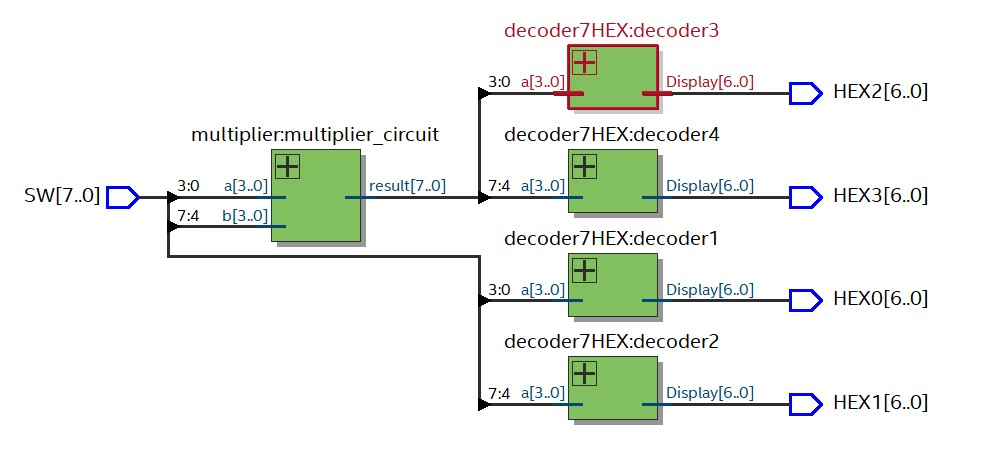
\includegraphics[scale = 0.5]{immagini/RTL_architecture_4.jpg}
	\caption{the RTL schematics of the overall circuit}       

\end{figure}
The converters used were the same of the previous parts, since their function is the same.
For implementing the multiplier 2 type of components were used: 4-bit adders (adder.vhd) and and arrays (and\textunderscore array.vhd).
The 4-bit adders are composed of 4 full adders and they do the intermediate addition, like the 7-segments converters the full adder components were reused from previous parts.
The and arrays perfoms the multiplication of one factor by one bit of the other.
\begin{figure}[h]
	\centering
	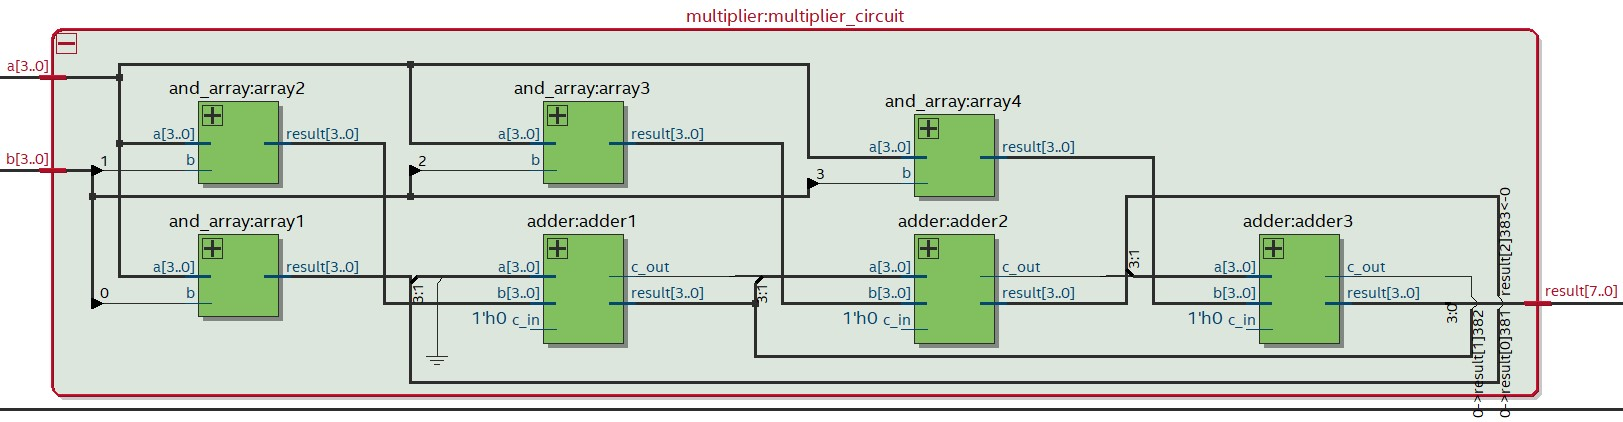
\includegraphics[scale = 0.4]{immagini/RTL_multiplier.jpg}
	\caption{the RTL schematics of the multiplier component}       

\end{figure}
\subsection{Testing the circuit}
The testing of single components was done manually using Modelsim since all of the components were either reused from previous points or trivial. \newline
A testbench was used for testing the overall circuit, this testbench tests all the possible 256 pairs of inputs.
Despite the big number of possible pairs reading the test result is practical as the operation of the circuit is just a simple multiplication. \newline
Inputs were generated procedurally through 2 nested for loops and they were provided with a 8-bit vector that simulated the switches vector.\newline
The tests of circuit done on the DE10 board confirmed the Modelsim simulations.



\end{document}
